\section{Auswahl einer geeigneten Untermenge an Parametern}

\subsection{Vorgehen}
Um eine geeignete Untermenge an Parametern zu finden, haben wir die Relevanz der
Parameter evaluiert. Dafür sind wir wie folgt vorgegangen:

Die TMVA-Methoden geben selbst eine Rangliste in Bezug auf die Relevalnz der
Parameter aus. Um diese zu evaluieren, ließen wir die Trainingsalgorithmen
dreisig mal durchlaufen - jedes Mal mit einer Variable weniger und die
Reihenfolge des Entfernens entsprach der Rangliste. Jedes Mal wurde der AMS-Wert
protokoliert. Diese Methode werteten wir für das Liklihood-, das Fisher- und das
BDT-Verfahren aus.

Für das MLP-Verfahren gingen wir wie folgt vor: Wir trainierten das neuronale
Netz dreisig mal und liesen jedes Mal einen anderen Parameter weg. Desto höher
der erreichte AMS-Wert war, desto irrelevanter bzw. sogar nachteiliger ist der
weggelassene Parameter. Gemäß des AMS-Werts lässt sich ebenfalls eine Rangliste
erstellen. Danach wurde so verfahren, wie im vorangehenden Abschnitt
beschrieben: Das Training wurde mit 30, dann mit 29, dann mit 29, \ldots
Parametern durchgeführt, wobei die Reihenfolge des Weglassens der erstellten
Rangliste entsprach.

Das beste vorgehen war allerdings Folgendes: Wir trainierten die Methoden
und liesen dabei jedes Mal einen anderen Paramerter weg. Der Parameter, dessen
Entfernen den höchsten AMS-Wert erreichte, wurde aus der Parametermenge
entfernt.
Dieses Vorgehen wurde wiederholt bis nur noch ein Parameter übrig war. Dafür
sind 465 Trainingszyklen notwendig. Aufgrund der langen Trainingszeit
haben wir dieses Vorgehen nicht bei der MLP-Methode verwendet.


\subsection{Auswertung}

Die Ergebnisse sind in Abbildung \ref{fig:ams_over_parameter_count} gezeigt.
Welche Parameteranzahl wir für jede Methode verwendet haben ist durch einen
senkrechten Strich gekennzeichent und liegt jeweils beim maximalen AMS-Wert.
Die Rangliste der Parameter und welche Parameter wir letztendlich benutzt haben,
steht in Tabelle \ref{table:parameter_ranking}.

Die Ergebnisse zeigen, dass bei der Likelihood- und bei der Fisher-Methode
unsere Rangliste der Parameter ein besseres Ergebnis liefert als die interne
Rangliste der TMVA-Methoden.

Ausschlaggebend bezüglich des AMS-Wertes ist die Verkleinerung der
Parametermenge lediglich bei der Likelihood-Methode. Allerdings bringt eine
reduzierte Parametermenge auch eine reduzierte Laufzeit des Algorithmus mit
sich, was insbesondere für die MLP-Methode nützlich ist, da sie eine lange
Trainigszeit erfordert.




%\usepackage{graphics} is needed for \includegraphics
\begin{figure}[htp]
\begin{center}
  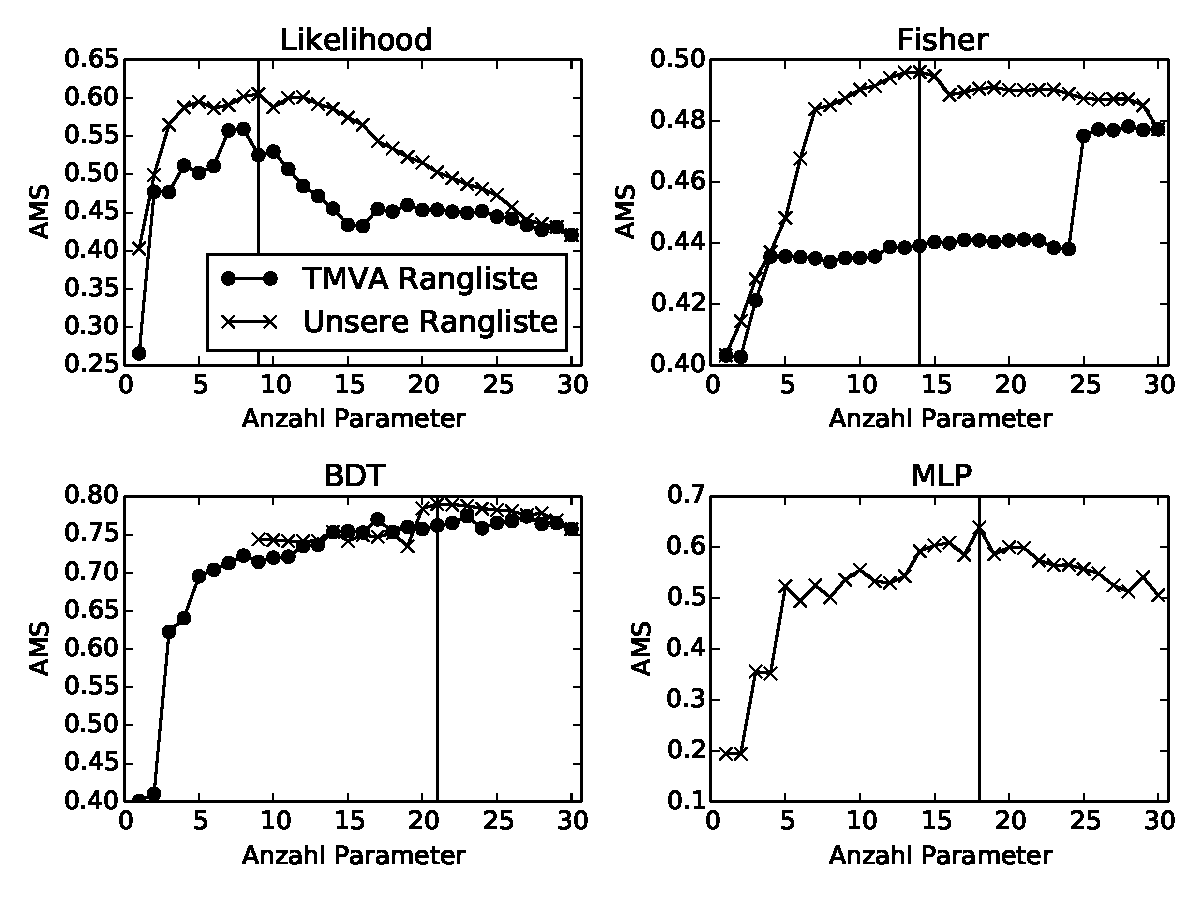
\includegraphics[width=\linewidth]{sections/subset_of_parameters/parameter_count_ranking_by_method.pdf}
  \caption[AMS über der Anzahl der Parameter]{AMS über der Anzahl der Parameter.}
  \label{fig:ams_over_parameter_count}
\end{center}
\end{figure}

\begin{table}
\caption{Bewertung der Parameter. Für die einzelnen Methoden nimmt die
Gewichtung der Parameter von oben nach unten ab. Für jede Methode ist durch
\mbox{"`-----"'} gekennzeichnet, welche Parameter nicht mehr verwendet werden.
Bei der BDT-Methode wurde unter den besten acht Parametern kein Ranking mehr
vorgenommen.}
\small
\hspace{-1cm}
\begin{tabular}{c|c|c|c}
Likelihood & Fisher & BDT & MLP \\
\hline
d\_mass\_transverse\_met\_lep & d\_mass\_transverse\_met\_lep & - & p\_jet\_num
\\
d\_mass\_vis & d\_pt\_ratio\_lep\_tau & - & d\_deltaeta\_jet\_jet \\ 
p\_tau\_pt & p\_lep\_pt & - & d\_mass\_MMC \\ 
d\_deltar\_tau\_lep & d\_mass\_vis & - & p\_jet\_leading\_pt \\ 
d\_pt\_ratio\_lep\_tau & d\_deltar\_tau\_lep & - & d\_mass\_transverse\_met\_l \\ 
p\_met & d\_pt\_h & - & p\_jet\_leading\_eta \\ 
p\_lep\_pt & p\_tau\_pt & - & d\_mass\_jet\_jet \\ 
p\_lep\_eta & d\_mass\_jet\_jet & - & p\_jet\_leading\_phi \\ 
d\_mass\_MMC & p\_met & d\_mass\_MMC & d\_pt\_h \\ 
----- & & & \\ 
p\_jet\_leading\_phi & d\_prodeta\_jet\_jet & d\_lep\_eta\_centrality & d\_mass\_vis \\ 
d\_met\_phi\_centrality & p\_jet\_subleading\_pt & p\_jet\_subleading\_phi & p\_jet\_subleading\_phi \\ 
p\_tau\_phi & p\_lep\_phi & p\_tau\_pt & d\_prodeta\_jet\_jet \\ 
p\_met\_phi & d\_mass\_MMC & d\_mass\_vis & p\_jet\_subleading\_pt \\ 
p\_tau\_eta & d\_deltaeta\_jet\_jet & p\_tau\_phi & p\_tau\_pt \\ 
 & ----- & & \\ 
p\_jet\_subleading\_pt & d\_lep\_eta\_centrality & p\_met\_sumet & p\_met\_phi \\ 
d\_pt\_tot & p\_jet\_leading\_phi & p\_lep\_pt & p\_jet\_all\_pt \\ 
p\_jet\_subleading\_eta & p\_jet\_leading\_eta & p\_lep\_phi & p\_met\_sumet \\ 
d\_prodeta\_jet\_jet & d\_sum\_pt & p\_jet\_subleading\_pt & p\_tau\_eta \\ 
 & & & ----- \\ 
p\_jet\_subleading\_phi & p\_jet\_subleading\_eta & p\_jet\_subleading\_eta & p\_met \\ 
p\_met\_sumet & p\_tau\_phi & d\_pt\_tot & d\_met\_phi\_centrality \\ 
d\_deltaeta\_jet\_jet & p\_met\_phi & p\_jet\_subleading\_eta & d\_pt\_ratio\_lep\_tau \\ 
 & & ----- & \\ 
d\_mass\_jet\_jet & p\_jet\_leading\_pt & p\_jet\_subleading\_phi & p\_tau\_phi \\ 
d\_lep\_eta\_centrality & p\_tau\_eta & p\_jet\_subleading\_pt & p\_jet\_subleading\_eta \\ 
p\_lep\_phi & p\_met\_sumet & d\_pt\_h & p\_lep\_phi \\ 
p\_jet\_num & p\_jet\_num & p\_met & d\_pt\_tot \\ 
d\_pt\_h & d\_pt\_tot & d\_prodeta\_jet\_jet & p\_lep\_eta \\ 
d\_sum\_pt & p\_lep\_eta & p\_lep\_pt & d\_sum\_pt \\ 
p\_jet\_leading\_pt & p\_jet\_subleading\_phi & d\_pt\_tot & d\_lep\_eta\_centrality \\ 
p\_jet\_all\_pt & p\_jet\_all\_pt & p\_met\_phi & p\_lep\_pt \\ 
p\_jet\_leading\_eta & d\_met\_phi\_centrality & p\_lep\_phi & d\_deltar\_tau\_lep

\end{tabular}
\label{table:parameter_ranking}
\end{table}